\begin{center}
    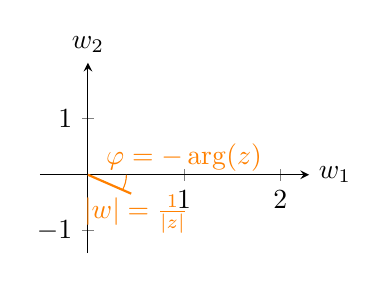
\begin{tikzpicture}
        [
            scale = 1.0,
            >=latex
        ]
        \begin{axis}[
            xmin=-0.5,
            xmax=2.3,
            ymin=-1.4,
            ymax=2,
            width=5cm,
            height=4cm,
            axis x line=middle, 
            axis y line=middle, 
            xtick={0, 1, 2},
            xticklabels={$0$, $1$, $2$},
            ytick={-1, 0, 1},
            x label style={anchor=west},
            xlabel={$w_1$}, 
            y label style={anchor=south},
            ylabel={$w_2$}
        ]
        
        \addplot[orange, thick, domain=0:0.45] {-0.75*x};
        \draw[orange] (0.4, 0) arc[start angle=0, end angle=-28, radius=0.4cm];
        \node[orange] at (1, 0.3) {$\varphi = -\arg(z)$};
        
        \node[orange] at (0.5, -0.7) {$|w| = \frac{1}{|z|}$};

        \end{axis}
    \end{tikzpicture}
\end{center}